%%%%% Document Setup %%%%%%%%

\documentclass[12pt, twocolumn]{revtex4}    % Font size (12pt) and column number (one or two).

\usepackage{times}  % Times New Roman font type

\usepackage{natbib}

\usepackage[a4paper, left=2.5cm, right=2.5cm,
 top=2.5cm, bottom=2.5cm]{geometry}       % Defines paper size and margin length

\renewcommand{\baselinestretch}{1.15}     % Defines the line spacing

\usepackage[font=small,
labelfont=bf]{caption}                      % Defines caption font size and caption title bolded

\usepackage{graphics,graphicx,epsfig,ulem}	% Makes sure all graphics works
\usepackage{amsmath}                        % Adds mathematical features for equations
\usepackage{float}

\usepackage{etoolbox}                       % Customise date to preferred format
\makeatletter
\patchcmd{\frontmatter@RRAP@format}{(}{}{}{}
\patchcmd{\frontmatter@RRAP@format}{)}{}{}{}
\renewcommand\Dated@name{}
\makeatother

\def\thesection{\arabic{section}}

\def\bibsection{\section*{References}}        % Position reference section correctly

%%%%% Document %%%%%
\begin{document}                     


\title{A Model for the Evolution of Quasars} 
\date{Submitted: \today{}}
\author{Joseph Carter}
\affiliation{\normalfont Level 4 Project, MPhys Physics with Astronomy\\ Supervisor: Professor T. Theuns\\ Department of Physics, Durham University}

%\begin{abstract}              
 
%Abstract abstract abstract abstract abstract abstract abstract abstract abstract abstract abstract abstract abstract abstract %abstract abstract abstract abstract abstract abstract abstract abstract abstract abstract abstract abstract abstract abstract %abstract abstract abstract abstract abstract abstract abstract abstract abstract abstract abstract abstract abstract abstract %abstract abstract abstract abstract abstract abstract abstract abstract abstract abstract abstract abstract 

%\end{abstract}


\maketitle
%\thispagestyle{plain} % produces page number for front page
\onecolumngrid


\tableofcontents
\newpage
\twocolumngrid
%\let\toc@pre\relax
%\let\toc@post\relax


\section{Introduction}

A quasar is an extremely luminous active galactic nucleus, typically associated with a supermassive black hole (SMBH) at the center of a galaxy. The intense radiation emitted by a quasar is thought to be caused by gas falling into the black hole (BH), with luminosities ranging between $~10^{11} - 10^{15}L_\odot$. The evolution of these galaxies' dark matter halos is well understood, but how this relates to the formation and evolution of quasars is not as well understood.\par
The aim of this project is to develop a model for the formation and evolution of quasars using a model for galaxy formation which includes feedback from stars and accreting black holes. This paper describes how the relation between the growth of SMBHs and the growth of their host galaxies can be used to determine the rate at which quasars are formed in the universe.

\subsection{The EAGLE Simulations}

Unless stated otherwise, all of the plots in this paper were produced using data from the Virgo Consortium’s “Evolution and Assembly of GaLaxies and their Environments” simulation suite (EAGLE) \cite{EAGLE}. This is a set of cosmological hydrodynamical simulations which use a modified version of the GADGET smoothed particle hydrodynamics code \cite{GADGET}. All plots were produced using the Ref-L0100N1504 simulation. This simulation includes feedback from stars and AGN, so it is useful for paramaters such as the formation rate of quasars to be based on data from this simulation. Full details of the parameters used in the simulations can be found in the EAGLE paper.

\subsection{COLOSSUS}

Some plots in this paper were also produced using COLOSSUS \cite{COLOSSUS}. This is a python package for calculations related to cosmology, the large-scale structure of matter in the universe, and the properties of dark matter halos. In particular, it is used in this paper to produce galaxy halo mass functions. It is shown in fig.? that the mass functions produced by COLOSSUS are a good fit for mass functions produced using data from EAGLE.

\section{The Black Hole Mass - Halo Mass Relation}



\section{Images}

Random Latin text.

\onecolumngrid


\begin{figure}[H]
\centering
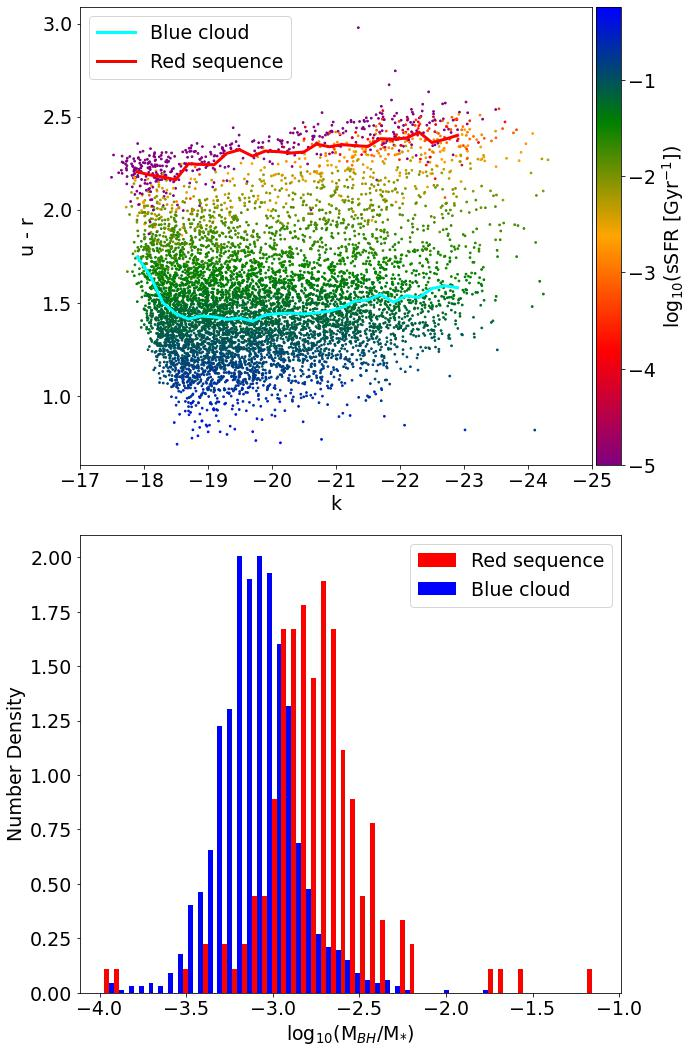
\includegraphics[width=11cm]{Plot_1.jpeg}
\caption{Top: u-r magnitude as a function of stellar mass for galaxies of mass greater than $10^9M_\odot$ at z=0. Individual galaxies are plotted as points, coloured by sSFR, using the colourbar to the right. Middle: Histogram of sSFR for galaxies of stellar mass between $10^{10} - 10^{10.5}M_\odot$ (the shaded region on the above plot). Bottom: Histogram of $M_{BH}/M_*$ for galaxies of stellar mass between $10^{10} - 10^{10.5}M_\odot$.}
\label{fig:1}
\end{figure}
\twocolumngrid


\newpage

Random Latin text.

\onecolumngrid


\begin{figure}[H]
\centering
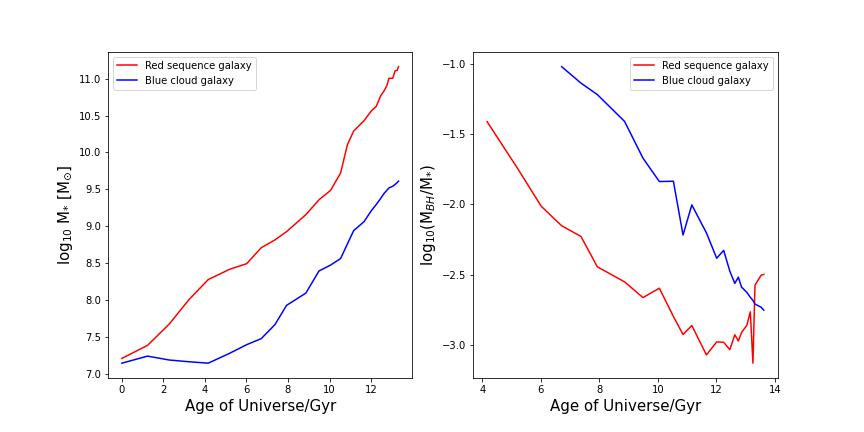
\includegraphics[width=14cm]{Plot_2.jpeg}
\caption{Plots of stellar mass, halo mass and black hole mass of two galaxies, one from the red sequence and one from the blue cloud, over cosmic time. The colour of the points show sSFR compared to the mean sSFR for central galaxies at that redshift. Colours from low to high sSFR: (cyan, blue, green, red, black).}
\label{fig:2}
\end{figure}
\twocolumngrid


\newpage

Random Latin text.

\onecolumngrid


\begin{figure}[H]
\centering
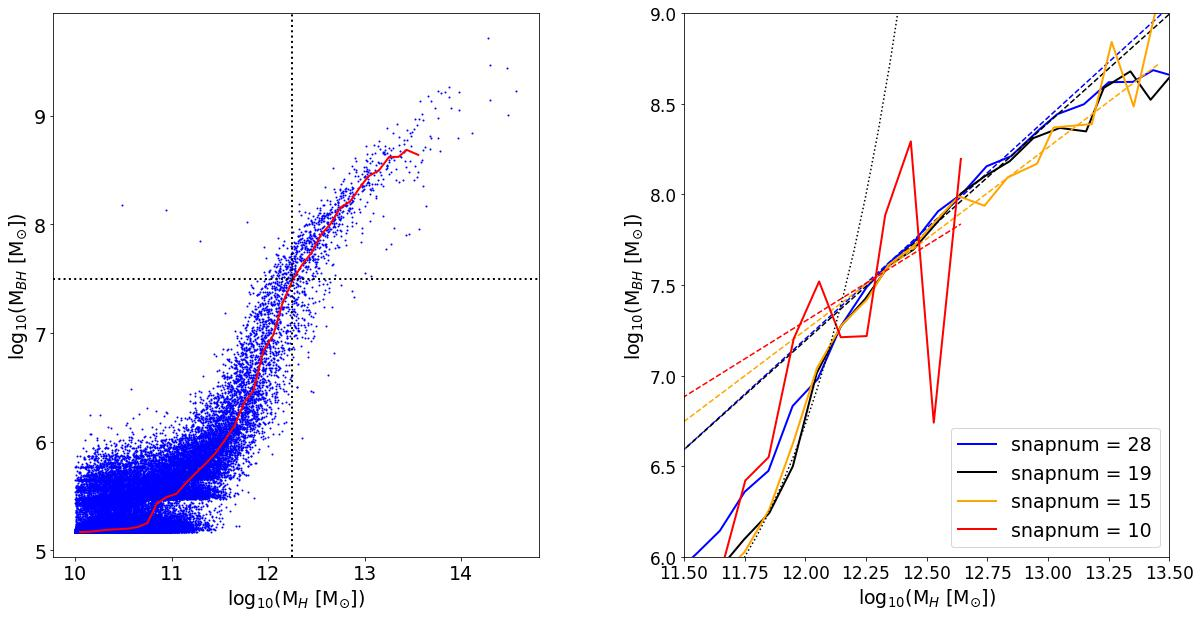
\includegraphics[width=17cm]{Plot_3.jpeg}
\caption{Left: Black hole mass - halo mass relation for central galaxies at z=0, the blue line shows median black hole mass. Right: Median black hole mass as a function of halo mass for central galaxies at snapnums 28, 19, 15, and 10 (equivalent to z = 0, 1, 2, and 4 respectively). Dashed lines show power law fits, the dotted line shows an exponential fit.}
\label{fig:3}
\end{figure}
\twocolumngrid


Random Latin text.

\onecolumngrid


\begin{figure}[H]
\centering
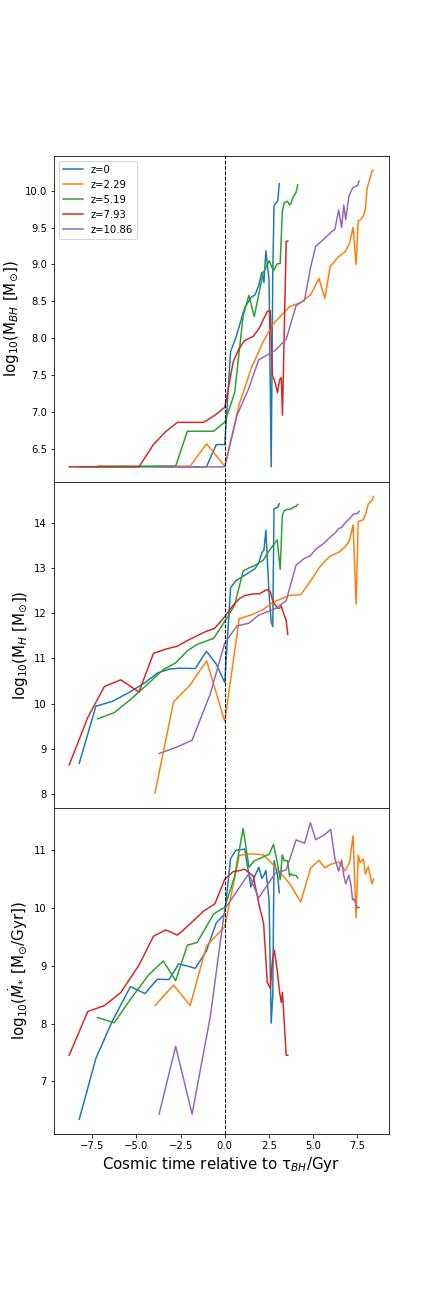
\includegraphics[width=11cm]{Plot_4.jpeg}
\caption{Black hole mass (top), Halo mass (middle), and sSFR (bottom) as a function of cosmic time relative to $\tau_{BH}$, where $\tau_{BH}$ is the time at which the black hole mass increases above $10^8M_\odot$.}
\label{fig:4}
\end{figure}
\twocolumngrid


Random Latin text.

\onecolumngrid


\begin{figure}[H]
\centering
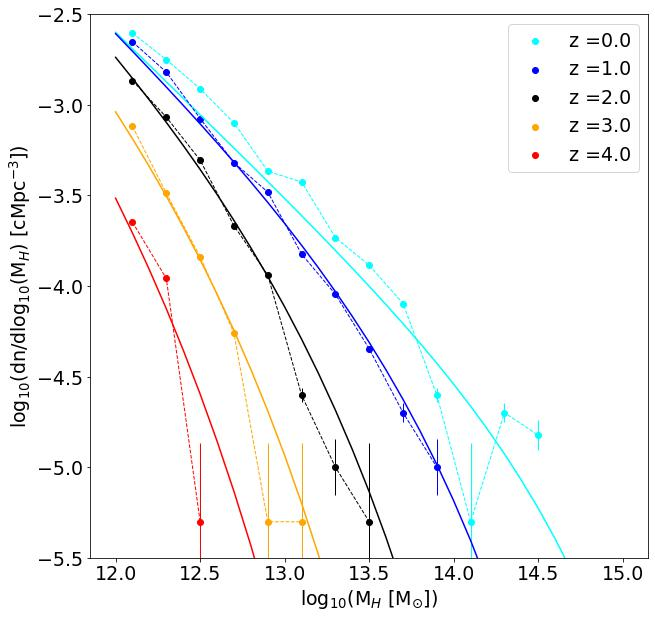
\includegraphics[width=\linewidth]{Mass_Function.jpeg}
\caption{Galaxy halo mass functions for galaxies of halo mass greater than $10^{12}M_\odot$ between z=0 and z=4. The dashed lines show mass functions from EAGLE, filled lines show mass functions from COLOSSUS.}
\label{fig:5}
\end{figure}
\twocolumngrid


Random Latin text.

\onecolumngrid


\begin{figure}[H]
\centering
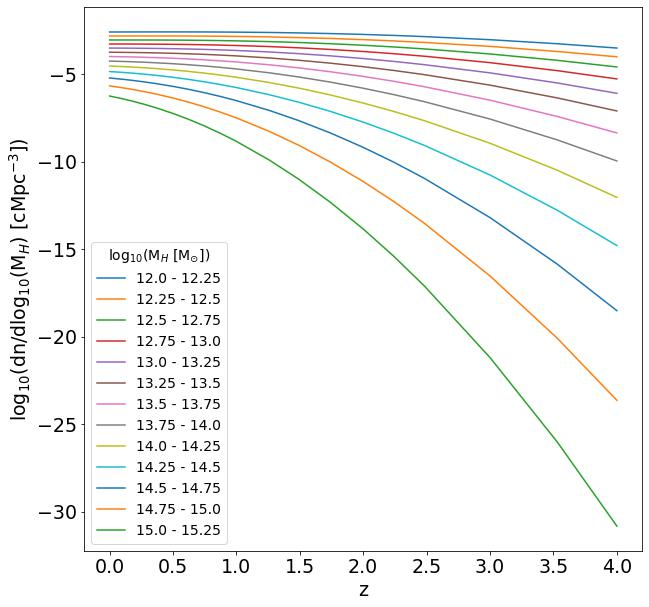
\includegraphics[width=\linewidth]{Mass_Function_2.jpeg}
\caption{Galaxy halo mass function as a function of redshift for galaxies of halo mass greater than $10^{12}M_\odot$. Produced using COLOSSUS.}
\label{fig:6}
\end{figure}
\twocolumngrid


Random Latin text.

\onecolumngrid


\begin{figure}[H]
\centering
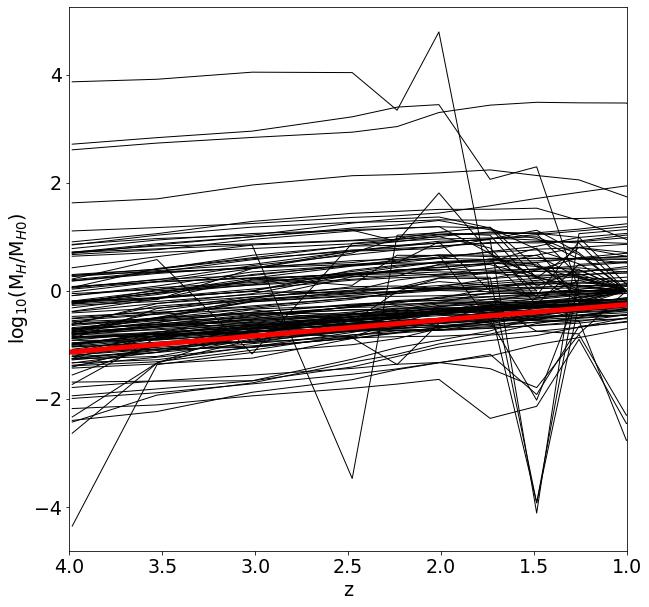
\includegraphics[width=\linewidth]{Plot_5.jpeg}
\caption{$M_H/M_{H0}$ as a function of redshift for central galaxies which cross the $10^{12}M_\odot$ halo mass threshold at z=2. The red line shows $M_H/M_{H0}$ as described by equation (?).}
\label{fig:7}
\end{figure}
\twocolumngrid


\onecolumngrid


\begin{figure}[H]
\centering
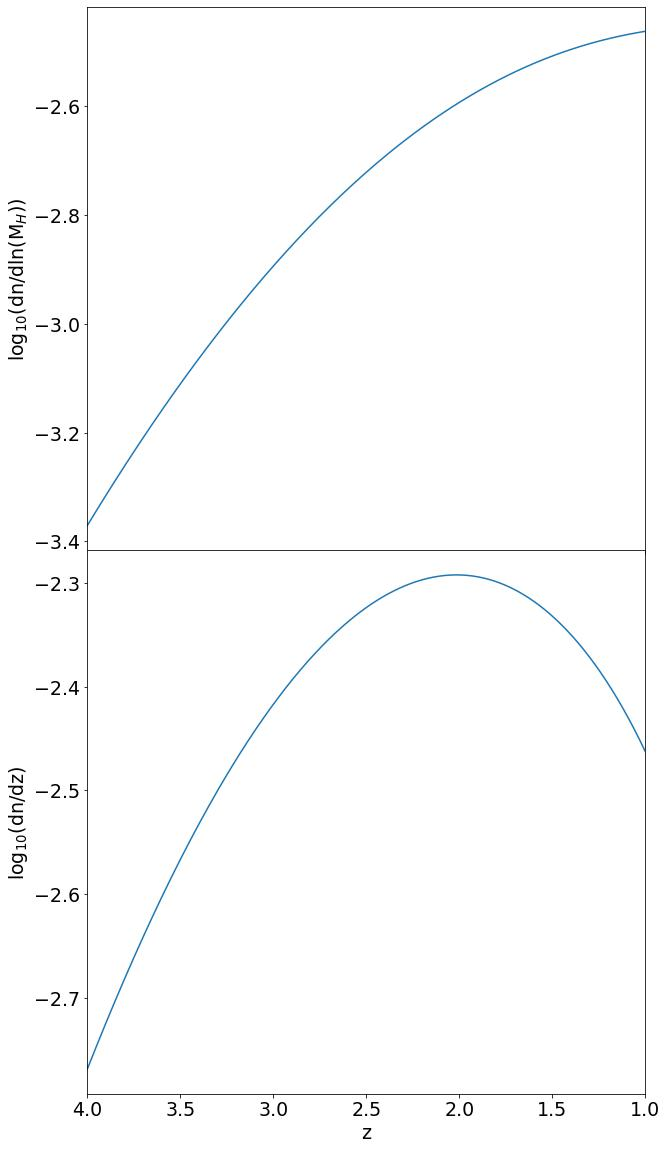
\includegraphics[width=12cm]{Plot_6.jpeg}
\caption{Top: Galaxy halo mass function as a function of redshift for galaxies of mass $10^{12}M_\odot$ produced using COLOSSUS. Bottom: Formation rate of halos of mass greater than $10^{12}M_\odot$ as a function of redshift, calculated using equation (?). This appears to peak at z=2.}
\label{fig:8}
\end{figure}
\twocolumngrid


\section{Section heading}

Duis eget tellus tortor. Cum sociis natoque penatibus et magnis dis parturient montes, nascetur ridiculus mus. In tellus nulla, sodales eu pulvinar at, accumsan quis magna. Nunc sed lacus diam. Nam enim mauris, imperdiet ut egestas quis, tincidunt at odio. Ut viverra nulla at libero dictum aliquet. Suspendisse lacus lacus, imperdiet nec elit nec, ullamcorper facilisis ex. \cite{Ikea} \cite{EAGLE}

\subsection{Subsection heading}

Proin sit amet mauris tincidunt, consectetur nisi ultrices, dapibus elit. Nullam vitae faucibus odio, pharetra ultrices tortor. Class aptent taciti sociosqu ad litora torquent per conubia nostra, per inceptos himenaeos. 

\section{Conclusions}
Donec finibus, tellus sit amet luctus sodales, lectus ante accumsan ligula, at condimentum lorem justo a sapien. Phasellus vel tortor vitae metus lacinia efficitur ac vel ex. Aenean eget congue leo. Aliquam cursus mauris sit amet arcu dignissim, vel condimentum nisi sodales. 

\bibliographystyle{unsrtnat}
\bibliography{citation.bib}

\end{document}